\subsection{Admin Controls} \label{subsec_admin_controls}
The admin controls exist to give administrators the ability to edit  important features of the chatbot, namely the classes, users and the math material itself.\newline\newline
It is important for them to be able to edit users or create new ones in the case of new students or teachers joining a class, or if passwords need to be reset or usernames changed. The reasoning behind allowing classes to be changed follows some of the same logic behind letting users be edited. Students and teachers leaving or joining classes in school means that they must be removed or added accordingly in the chatbot. Finally the math material presented itself must be able to be edited, as a change in the curriculum could lead to there being material missing in the chatbot or material that must be either edited or entirely removed. In all these cases it is imperative that the chatbot has the functionality to have the material changed in accordance to changes in the classroom.
\newline\newline
%The reason the ability to edit these features of the chatbot is exclusive to admins is because normal users with access to these features would be able to potentially severely hamstring it's effectiveness by wittingly or unwittingly sabotaging class lists and material. \newline\newline
When it comes to the general design of the admin controls, giving each major editable feature its own window would help an admin clearly identify that those are the three major editable features. Below is an example of a proposed design of the admin controls that starts on the users page.

\begin{figure}[H]
    \centering
    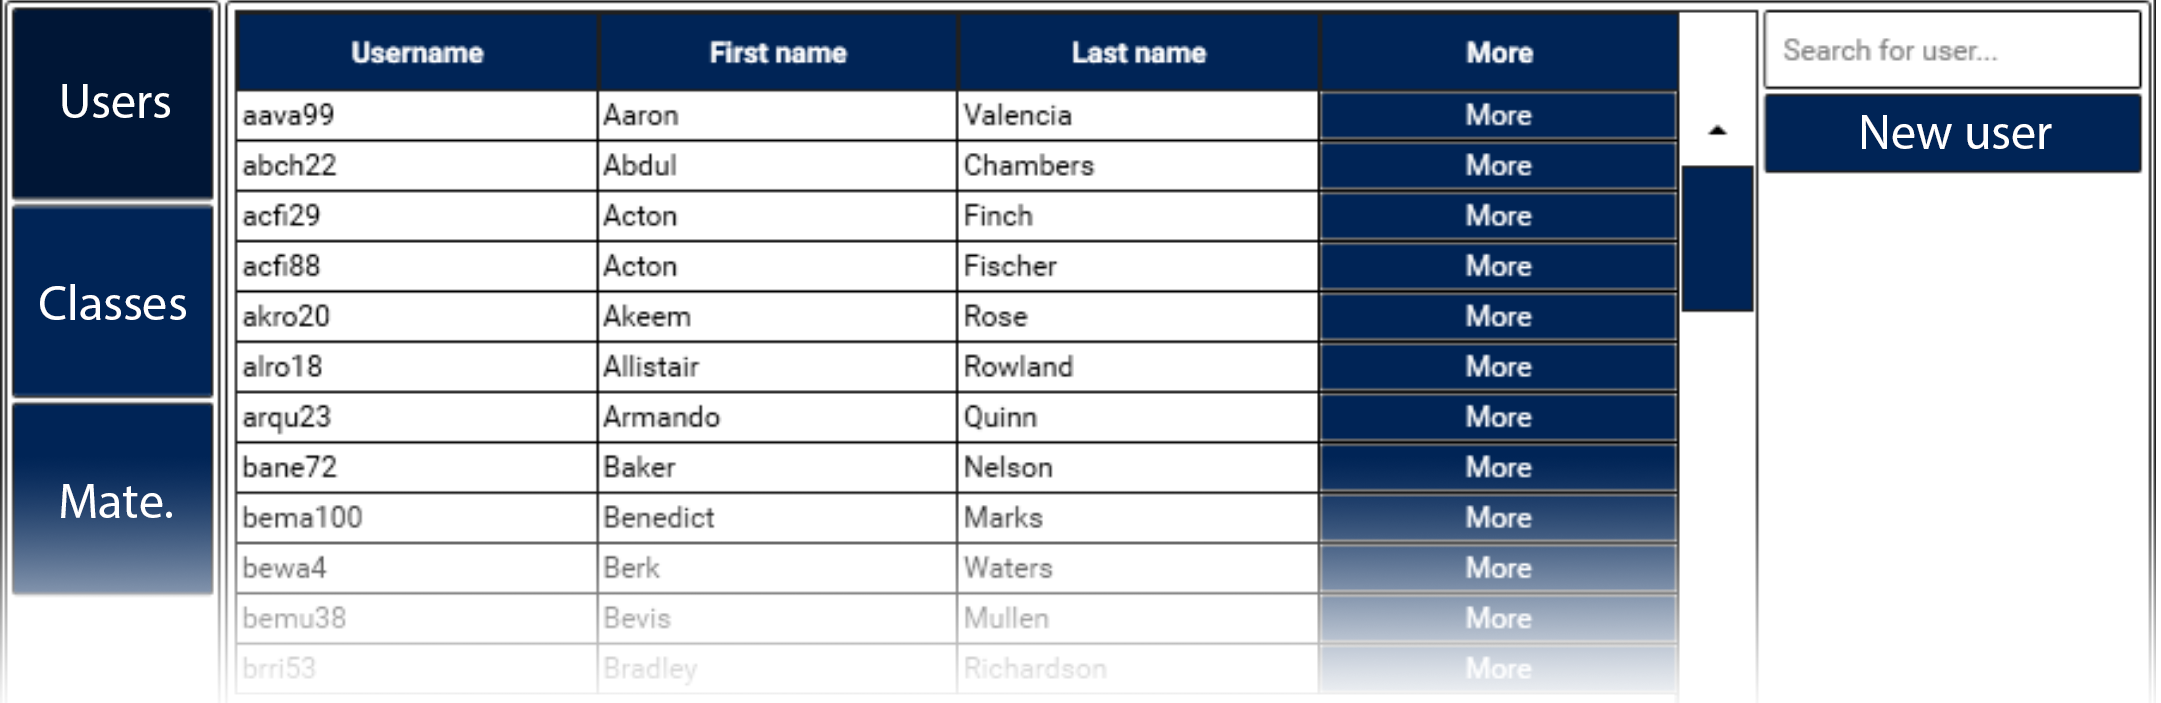
\includegraphics[width=0.6\textwidth]{figures/AdminControls.png}
    \caption{Example of proposed users window}
    \label{fig:user_interface}
\end{figure}

\noindent
As seen in the figure, there will be three named icons on the left that, when selected, take the admin to the initial page of the feature they represent. The current selected feature is indicated by the icon's colour being darkened. Each of the major tabs will have 3 sections. On the left will be the buttons leading to the other major editable features, in the center information will be presented, and on the right will be where search features as well as editing options will be found.
\newline\newline
For example, as previously mentioned, the figure is a proposed design for the users page. The center consists of a list of the usernames, as well as the first and last name of the user, organized alphabetically. This was chosen as it provides the admin with a clear overview of all the users registered by the application, as well as the ability to identify a user by their real name rather than their username, making it easier to identify which account belongs to which student or teacher. Included with each user entry is a more tab that gives access to the account editorial features, where passwords can be reset and roles assigned/changed. On the right is a button that allows for the creation of a new user, as well as a search feature to allow for quick location of a specific account.
\newline\newline
Both the classes and material page have a similar setup. The tabs leading to the other major features on the right, information presented as a list along with access to additional information and editorial options in the center, and search functionality and creational features on the right. 